\documentclass[12pt]{article}
\usepackage[english]{babel}

\usepackage[a4paper,top=2cm,bottom=2cm,left=3cm,right=3cm,marginparwidth=1.75cm]{geometry}

% Useful packages
\usepackage{amsmath}
\usepackage{graphicx}
\usepackage[colorlinks=true, allcolors=blue]{hyperref}
\usepackage{enumitem}

\usepackage{natbib}



\title{Discipline name: Embedded Systems}
\author{Bârsan Patricia-Diana, Christian Cezara-Cala}

\begin{document}

% \textbf{Smart Garden Irrigation System} where soil moisture level is monitored using sensors and a water pump is controlled for irrigation.

\begin{figure}
\centering

\includegraphics[width=0.8\linewidth]{images/image11.png}
\end{figure}

\maketitle

\newpage

\section{Introduction}

Terra Tech is a Smart Garden Irrigation System designed to efficiently manage watering schedules for your plants, addressing the challenge of over or under watering in traditional irrigation methods.\\


\hspace{1cm}Functionalities:
\begin{enumerate}[leftmargin=2cm]
\item \textbf{Plant Recognition with Webcam}: The system uses a webcam to capture images of the plant and using a trained AI model the plant species is detected
\item \textbf{Soil Moisture Sensing}: Using a soil moisture sensor it can be determined if the soil is dry or wet.
\item \textbf{DHT Sensor}: Using a DHT Sensor environmental data such as temperature and humidity are collected, providing insights into the plant’s growing conditions.
\item \textbf{Personalized routine}: Based on the plant type identified using AI the system offers a watering routine composed of a number of pumps and a number of seconds for each pump. It can also be personalized by the user.
\item \textbf{Manual Watering Control}: The user can decide when to start the watering routine for its plant using a dedicated mobile app. The watering is done through an water pump actuator and a tube.
\end{enumerate}

By integrating plant recognition technology and also an environmental sensor, Terra Tech optimizes the watering process for different plant species. This approach ensures that plants receive appropriate care for their specific needs. Also manual watering by a human cannot be that precise as the integrated water pump so the process will always be optimal for the plants.\\

\newpage 

\section{Description of the development board}

Used development board: Raspberry Pi 3 Model B+\\

\hspace{1cm}General Characteristics: 
\begin{itemize}[leftmargin=2cm]
    \item The Raspberry Pi 3 Model B+ is a compact single-board computer (SBC) developed by the Raspberry Pi Foundation.
    \item It features a Broadcom BCM2837B0, Cortex-A53 (ARMv8) 64-bit system-on-chip (SoC) @ 1.4GHz 1GB LPDDR2 SDRAM.
    \item The board includes onboard Wi-Fi (802.11b/g/n/ac) and Bluetooth 4.2, expanding connectivity options for various applications.
    \item It is equipped with a range of ports including HDMI, USB, Ethernet, and GPIO (General Purpose Input/Output) pins.
\end{itemize}

\begin{figure}[ht]
    \centering
    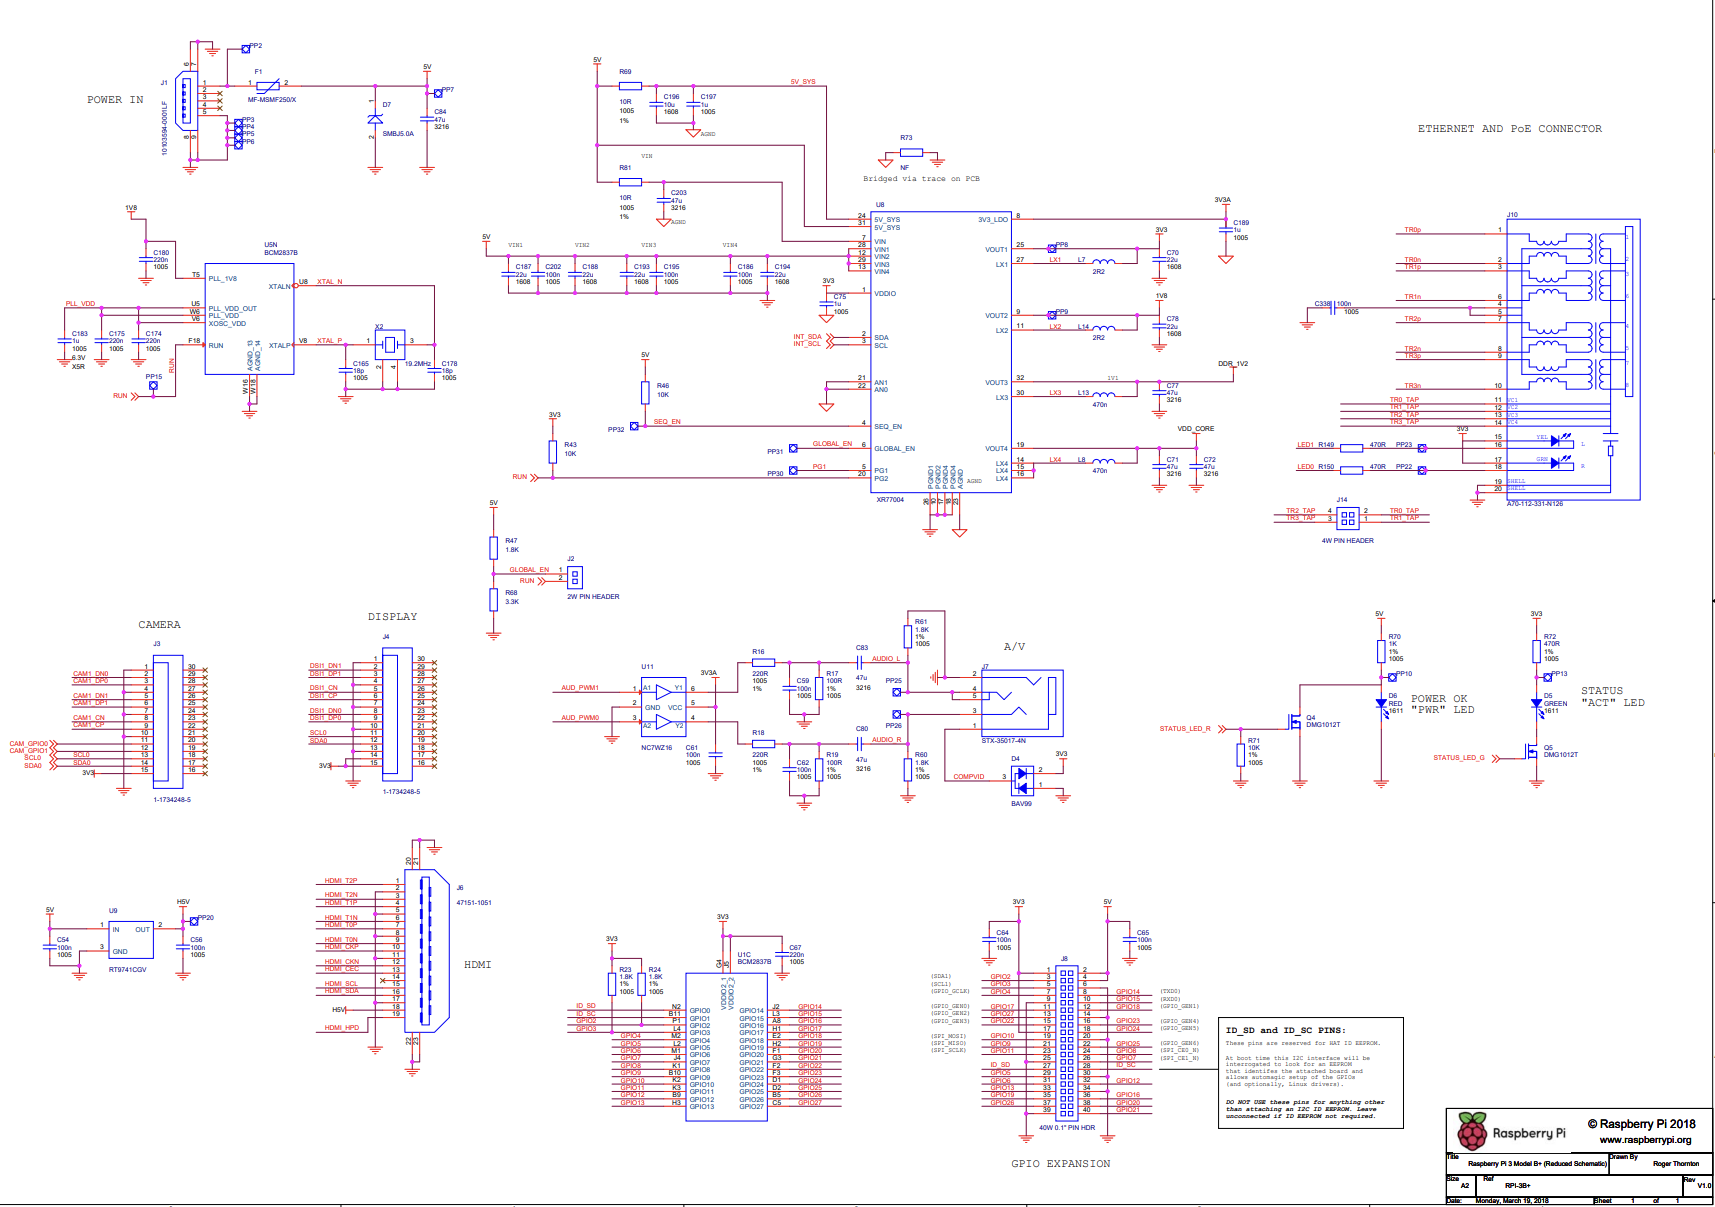
\includegraphics[width=0.9\textwidth]{images/image8.png}
    \caption{Raspberry Pi 3 Model B+ schematics}
    \label{fig:pic1}
\end{figure}  

\textbf{BCM2837B0} is manufactured by Broadcom and is the SoC used in the Raspberry Pi 3 Model B+. The underlying architecture of the BCM2837B0 is identical to the BCM2837 chip used in other versions.\\

\newpage

\begin{figure}[ht]
    \centering
    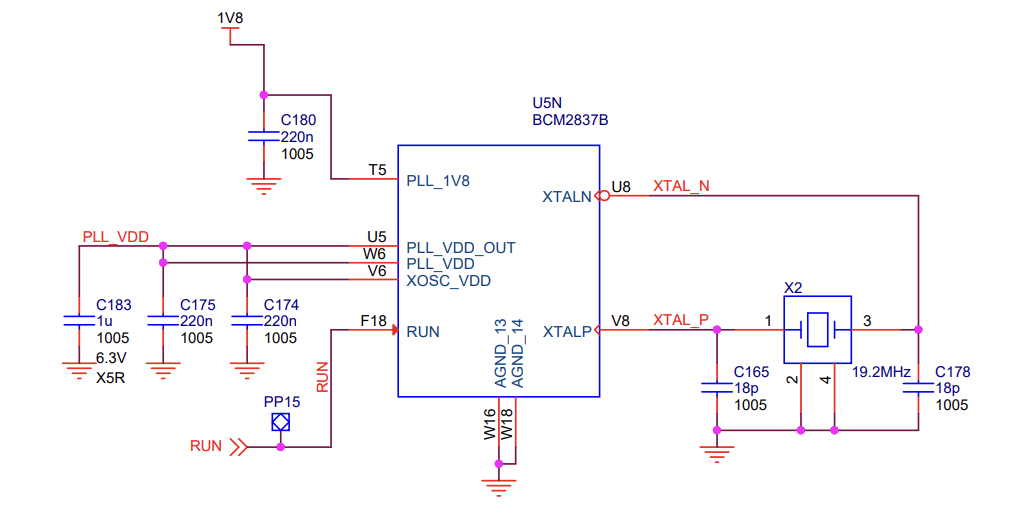
\includegraphics[width=0.9\textwidth]{images/image6.png}
    \caption{BCM2837B0}
    \label{fig:pic2}
\end{figure} 

The CPU used on Raspberry Pi 3 Model B+ is A 1.4GHz 64-bit quad-core \textbf{ARM Cortex-A53}\\


\begin{figure}[ht]
    \centering
    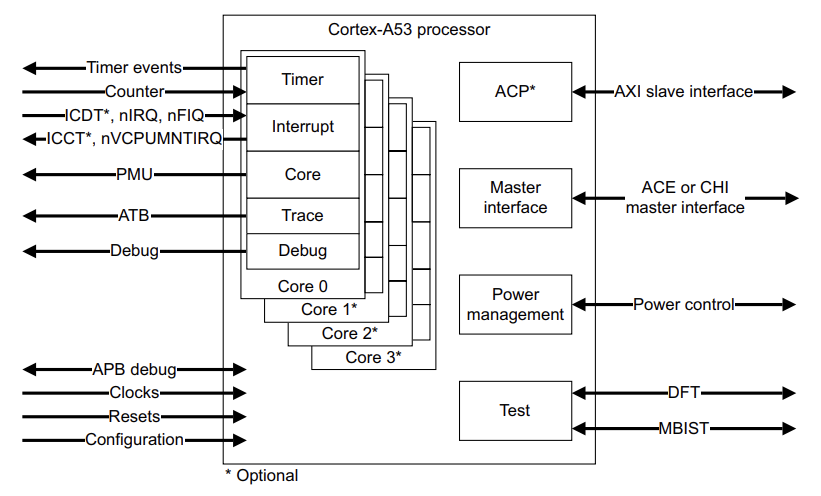
\includegraphics[width=0.9\textwidth]{images/image3.png}
    \caption{Cortex-A53 processor configuration}
    \label{fig:pic3}
\end{figure} 

\begin{figure}[ht]
    \centering
    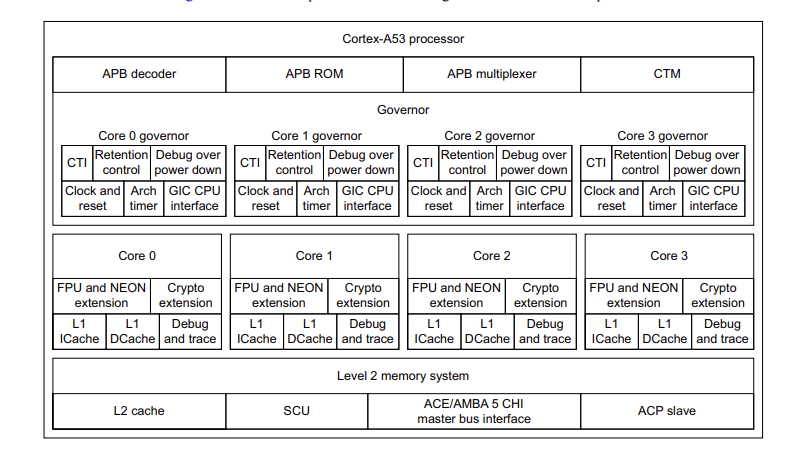
\includegraphics[width=0.75\textwidth]{images/image9.png}
    \caption{Cortex-A53 block diagram}
    \label{fig:pic4}
\end{figure} 

\newpage
\section{System Architecture}

\begin{figure}[ht]
    \centering
    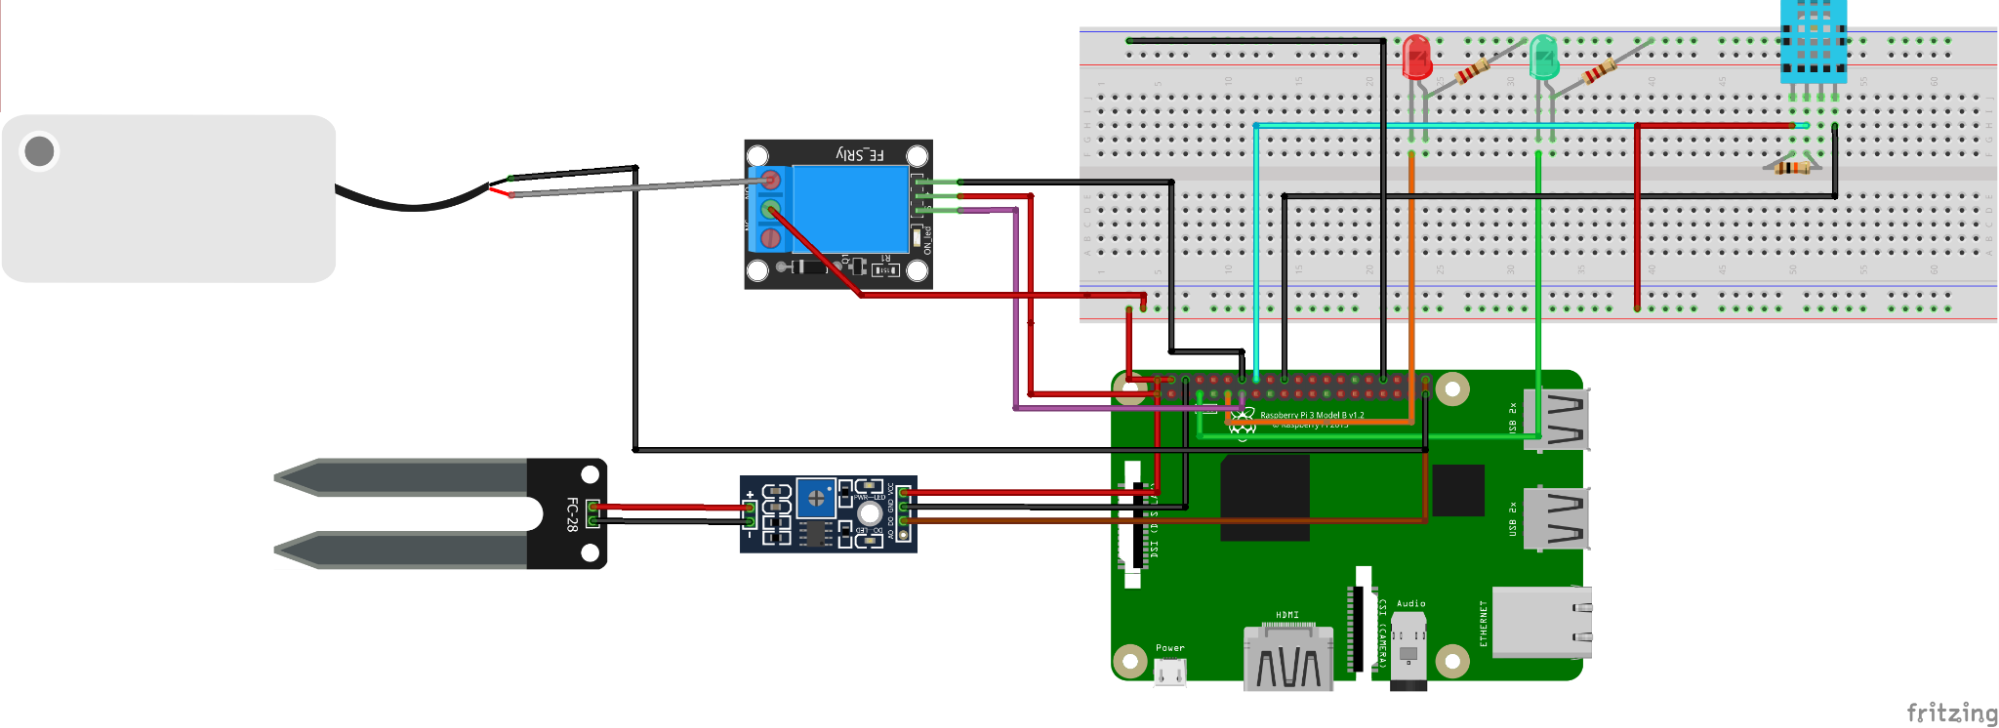
\includegraphics[width=0.7\textwidth]{images/image18.png}
    \caption{Breadboard view}
    \label{fig:pic5}
\end{figure} 

\begin{figure}[ht]
    \centering
    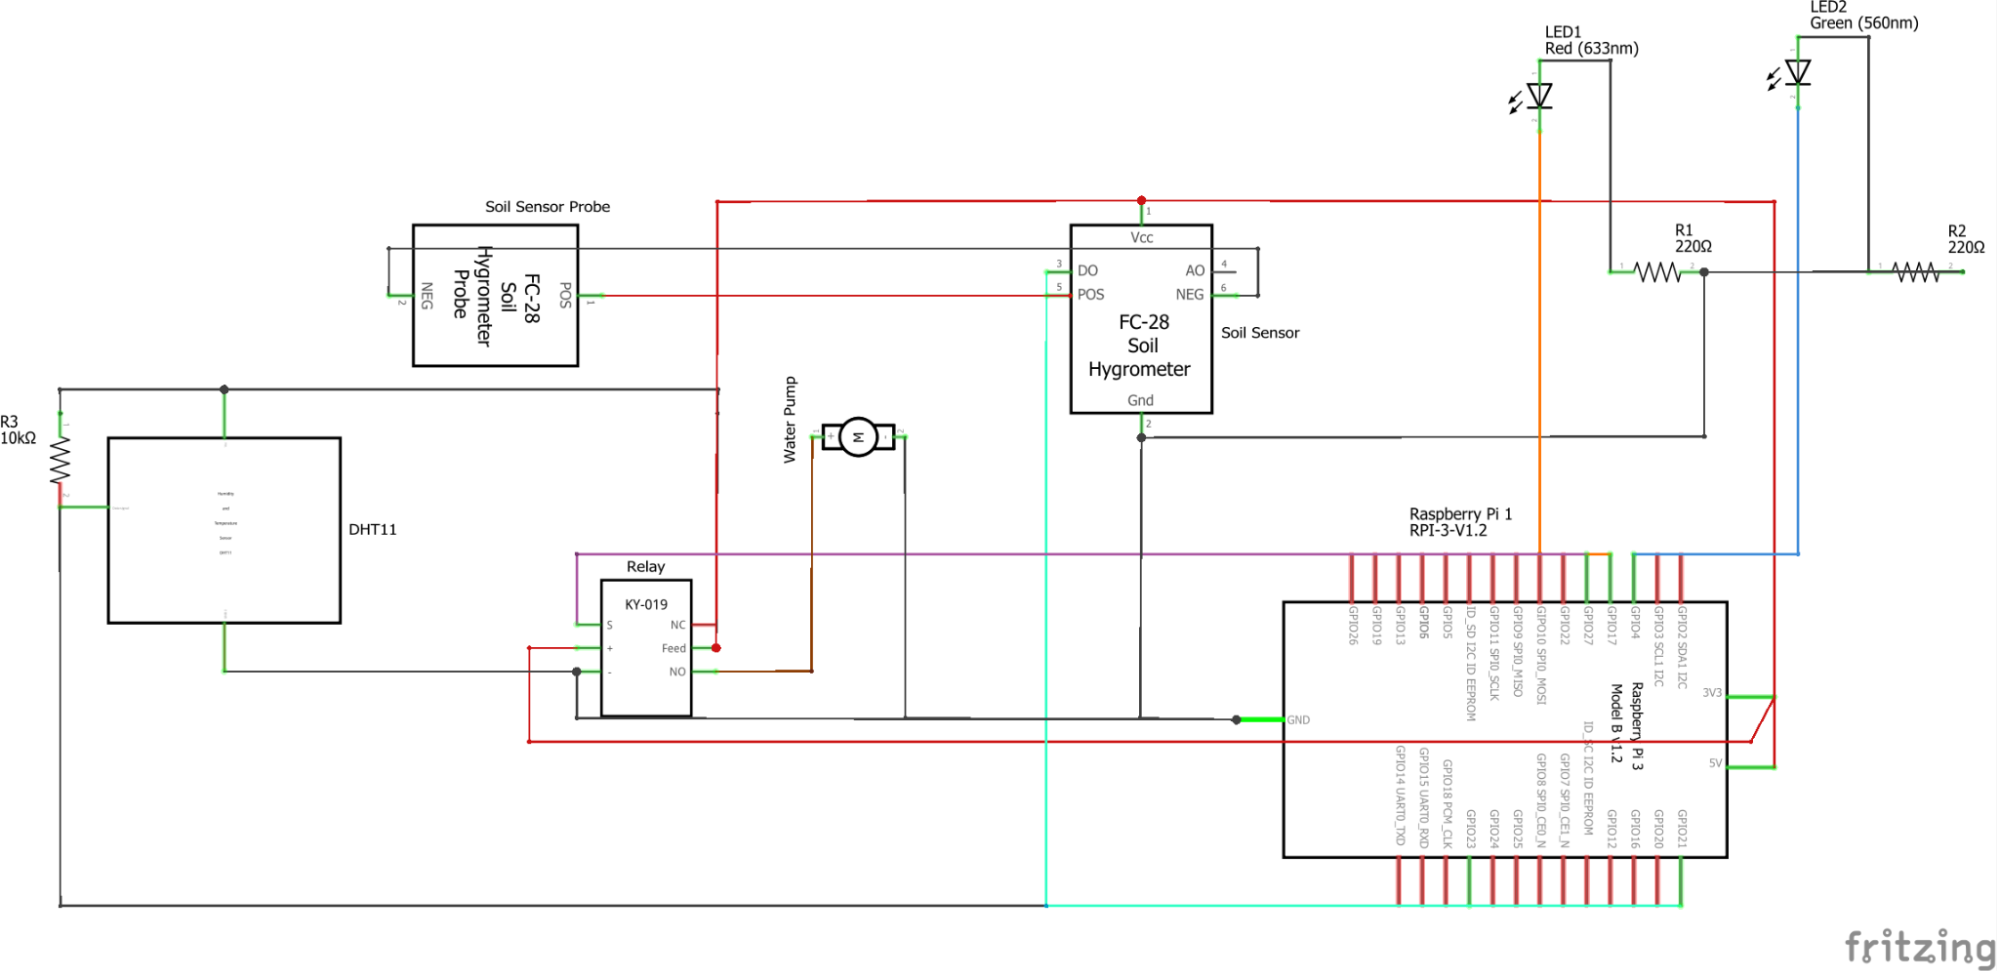
\includegraphics[width=0.7\textwidth]{images/image7.png}
    \caption{Schematic View}
    \label{fig:pic6}
\end{figure} 

\newpage

\begin{figure}[ht]
    \centering
    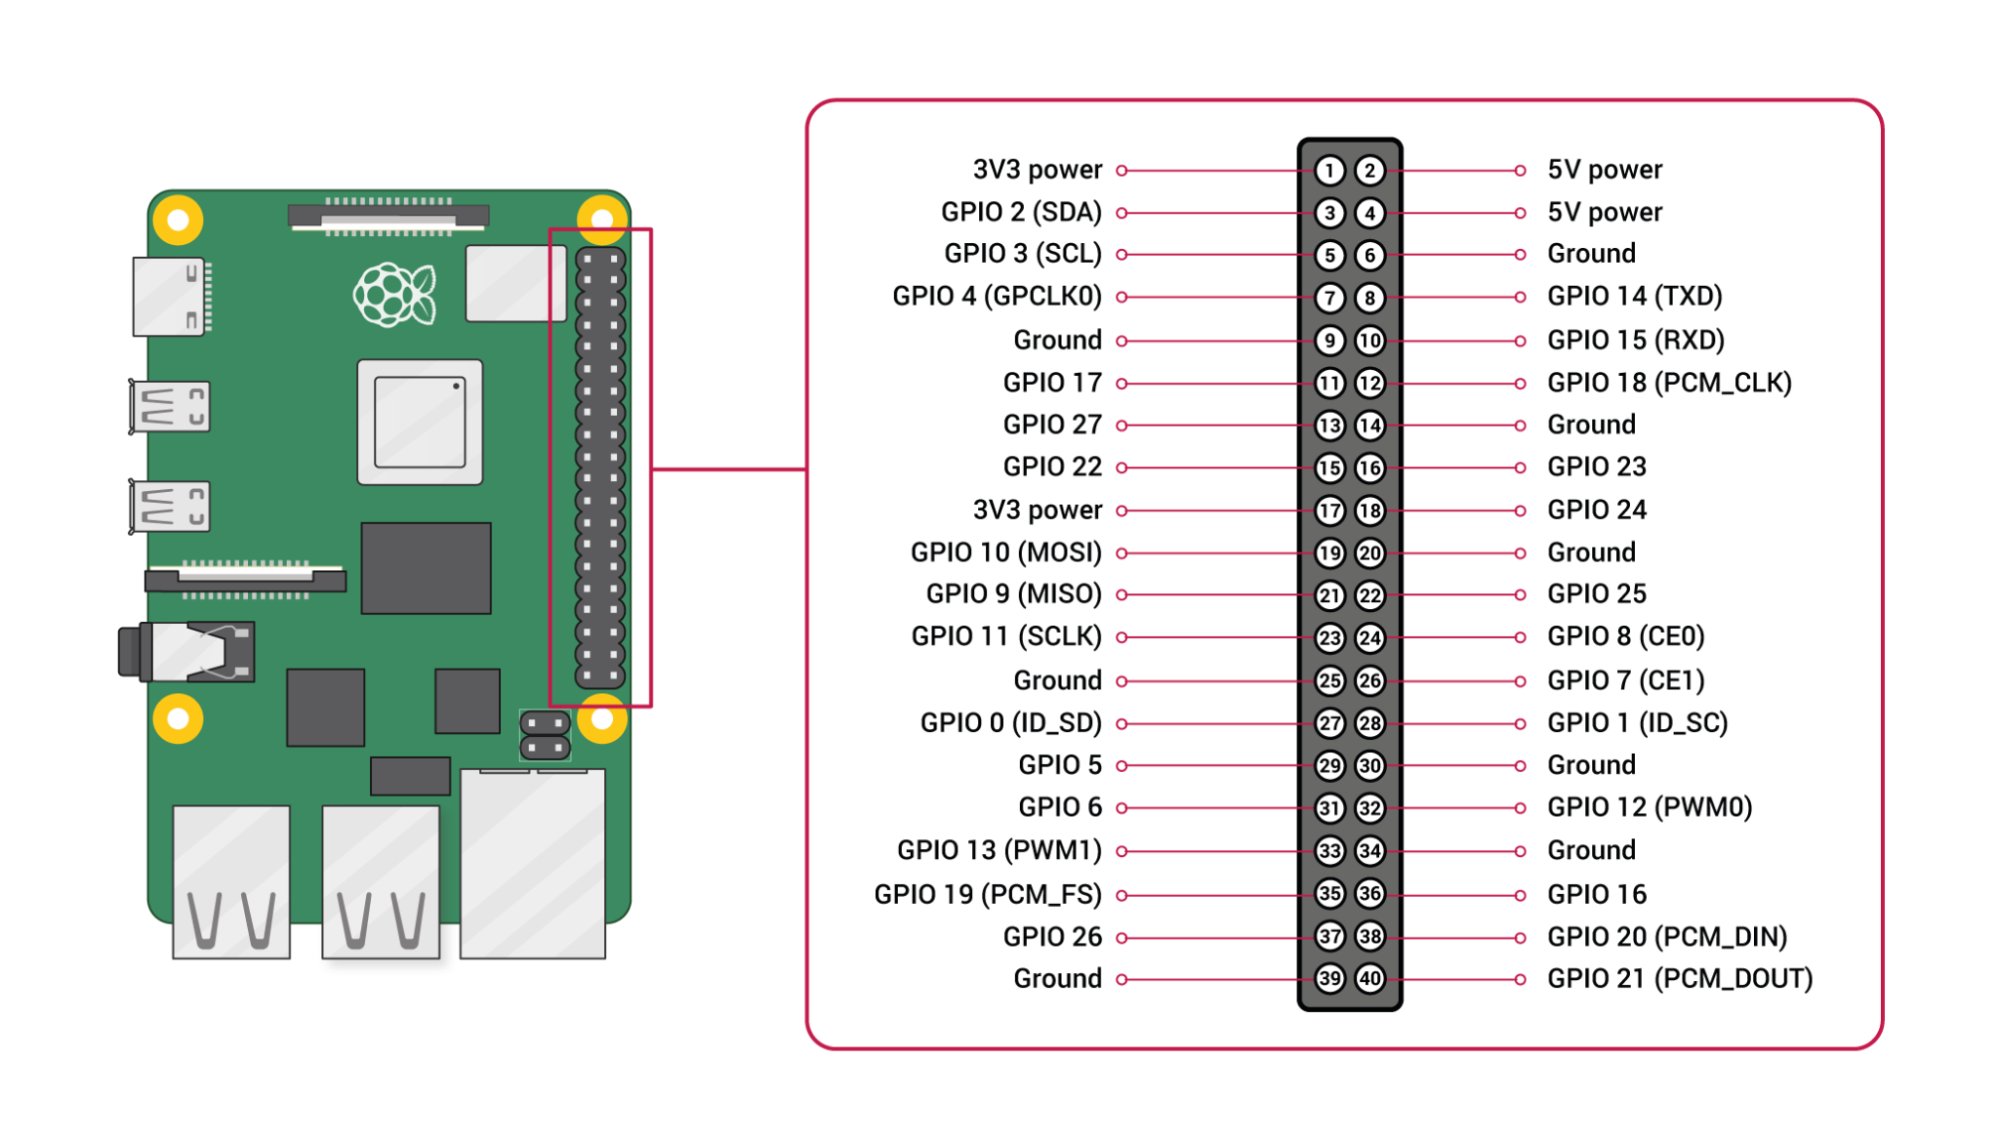
\includegraphics[width=0.9\textwidth]{images/image12.png}
    \caption{PIN Configuration of Raspberry Pi 3 Model B+}
    \label{fig:pic7}
\end{figure} 

Any of the GPIO pins can be designated in software as an input or output pin. In the project GPIO21 and GPIO27 were used as input, respectively output pins. To set the mode \textbf{GPIO.setmode(number, GPIO.IN/OUT)} was used.

\section{Sensors and actuators used}

\textbf{DHT11} is a commonly used \textbf{Temperature and Humidity sensor} that comes with a dedicated NTC to measure temperature and an 8-bit microcontroller to output the values of temperature and humidity as serial data.\\

\hspace{1cm}Specifications: 
\begin{itemize}[leftmargin=2cm]
    \item Operating Voltage: 3.3V to 5.5V
    \item Operating current: 0.3mA (measuring) 60uA (standby)
    \item Output: Serial data
    \item Temperature Range: 0°C to 50°C
    \item Humidity Range: 20\verb|% to 90%|
    \item Resolution: Temperature and Humidity both are 16-bit
    \item Accuracy: ±1°C and ±1\verb|%|
\end{itemize}

\newpage

\begin{figure}[ht]
    \centering
    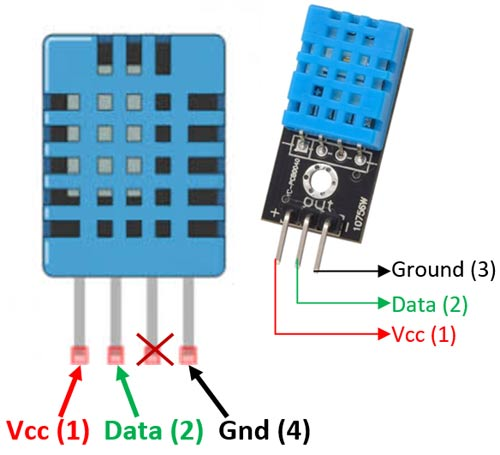
\includegraphics[width=0.6\textwidth]{images/image13.png}
    \caption{PIN Configuration for DHT11}
    \label{fig:pic8}
\end{figure} 

\begin{figure}[ht]
    \centering
    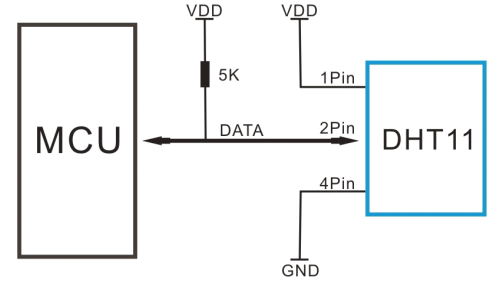
\includegraphics[width=0.6\textwidth]{images/image14.png}
    \caption{Block Diagram of DHT11}
    \label{fig:pic9}
\end{figure} 

\textbf{Soil Moisture Sensor} is commonly used \textbf{to measure the water content of soil}. It has a potentiometer, with which its sensibility level can be modified.\\

\hspace{1cm}Specifications: 
\begin{itemize}[leftmargin=2cm]
    \item Operating Voltage: 3.3V to 5.5V
    \item Operating current: <20 mA
    \item Output: both analog and digital
\end{itemize}

\begin{figure}[ht]
    \centering
    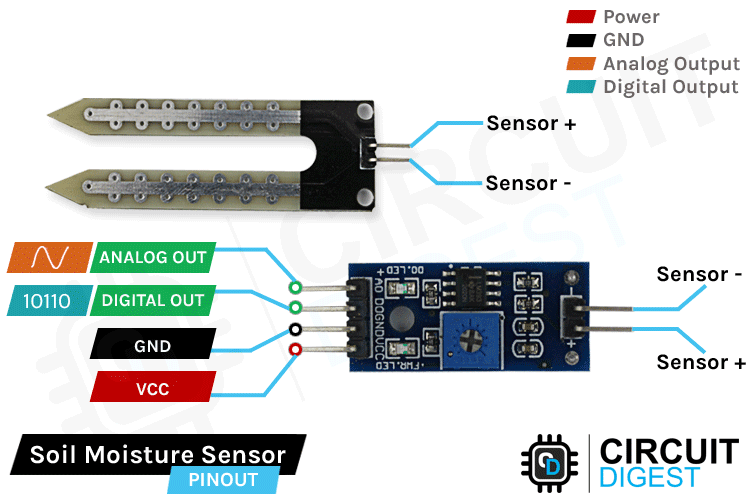
\includegraphics[width=0.6\textwidth]{images/image16.png}
    \caption{PIN Configuration for Soil Moisture Sensor}
    \label{fig:pic10}
\end{figure} 

\newpage
The probe has \textbf{two exposed conductive plates that will act as a variable resistor} whose resistance will vary depending on the water content in the soil. This resistance of the probe is inversely proportional to the soil moisture of the device.

\begin{figure}[ht]
    \centering
    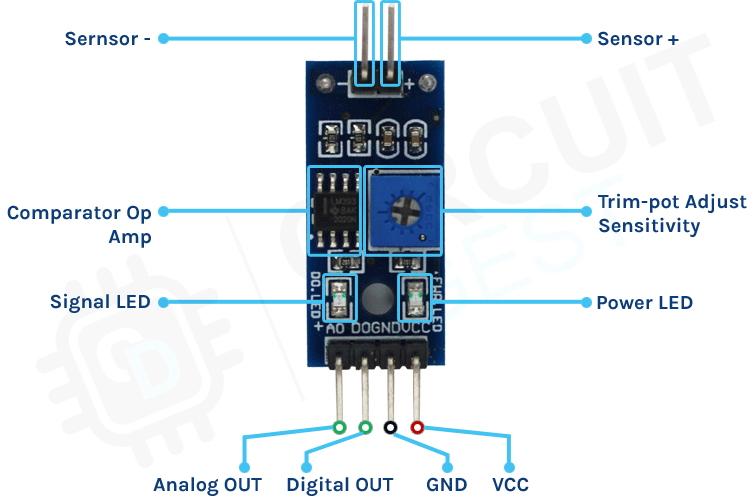
\includegraphics[width=0.55\textwidth]{images/image15.png}
    \caption{Soil Sensor Module}
    \label{fig:pic11}
\end{figure} 

\begin{figure}[ht]
    \centering
    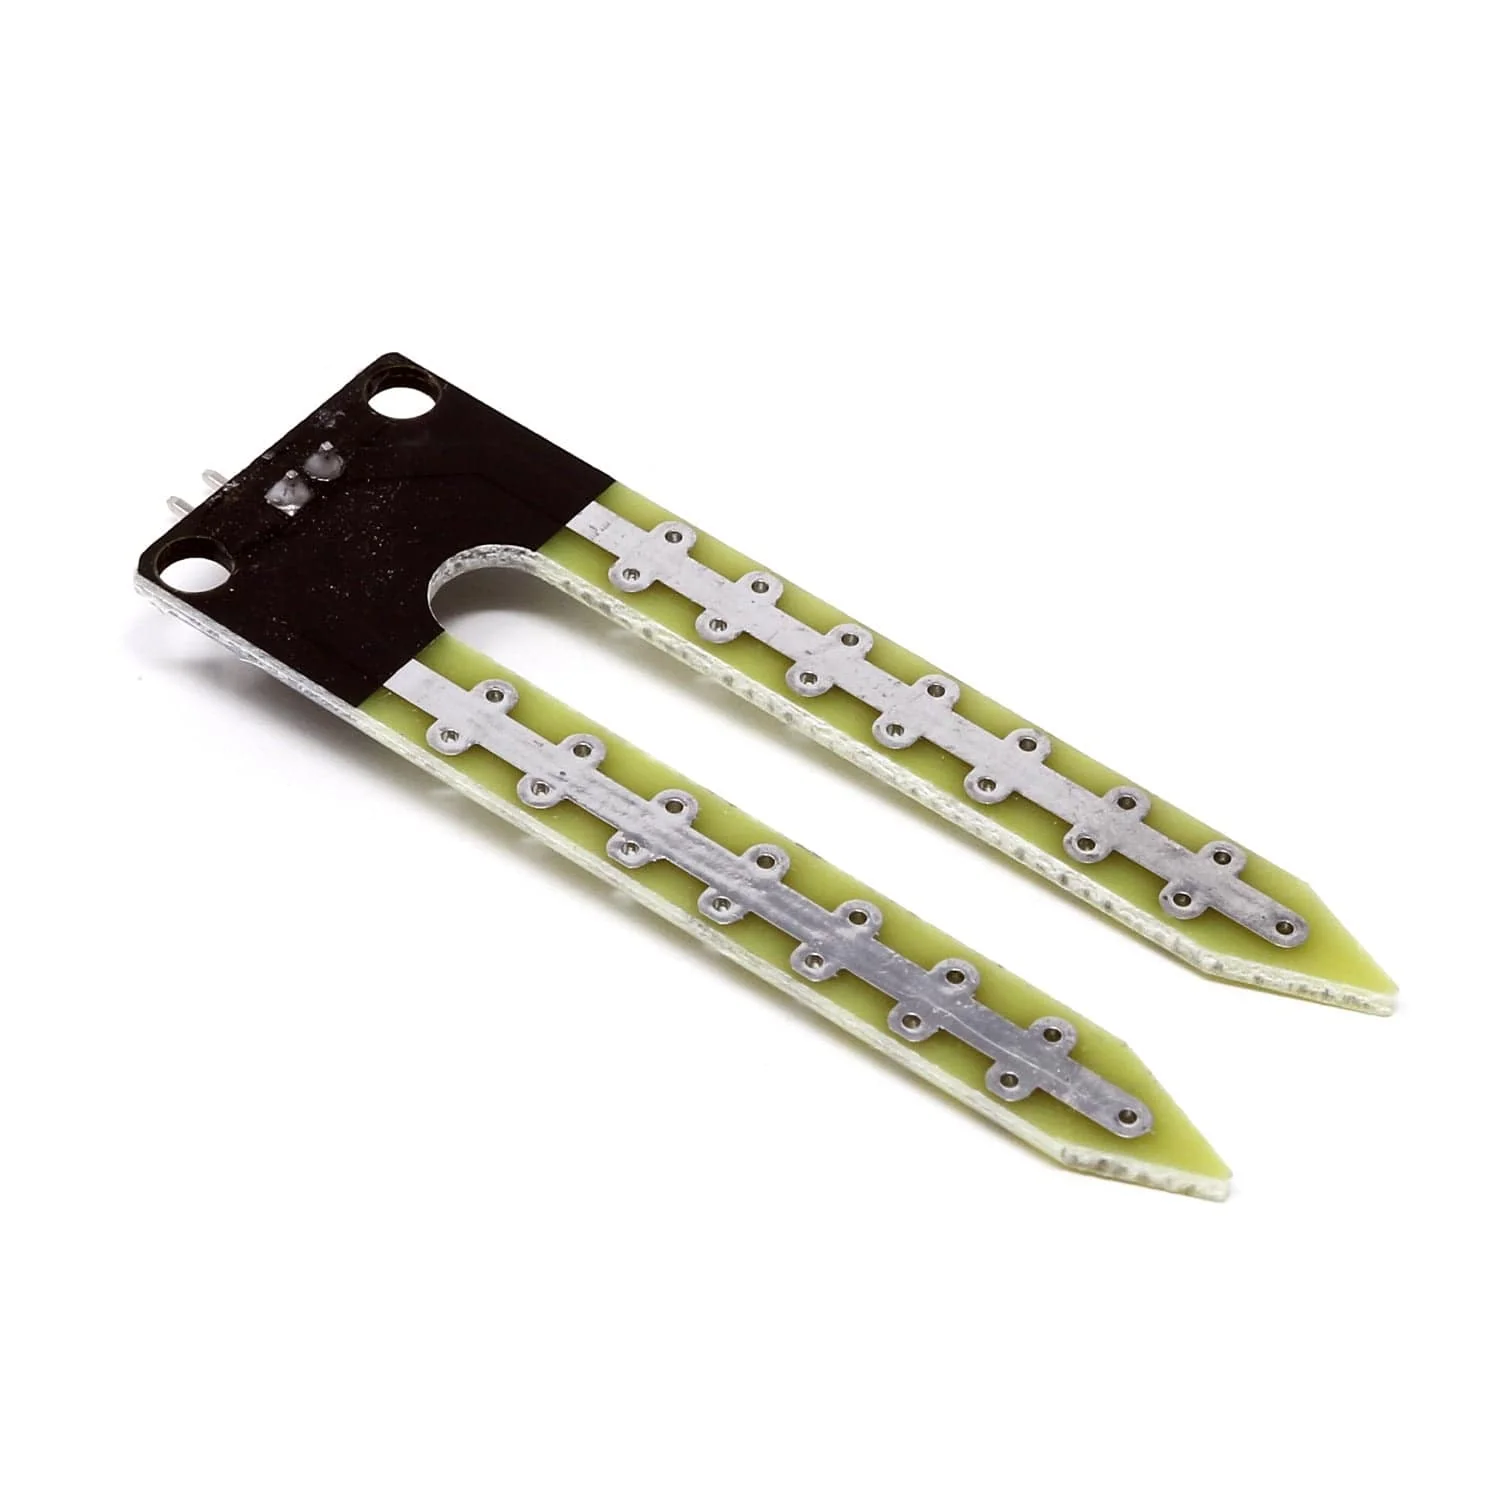
\includegraphics[width=0.27\textwidth]{images/image20.png}
    \caption{Soil Sensor Probe}
    \label{fig:pic12}
\end{figure} 

\newpage

\begin{figure}[ht]
    \centering
    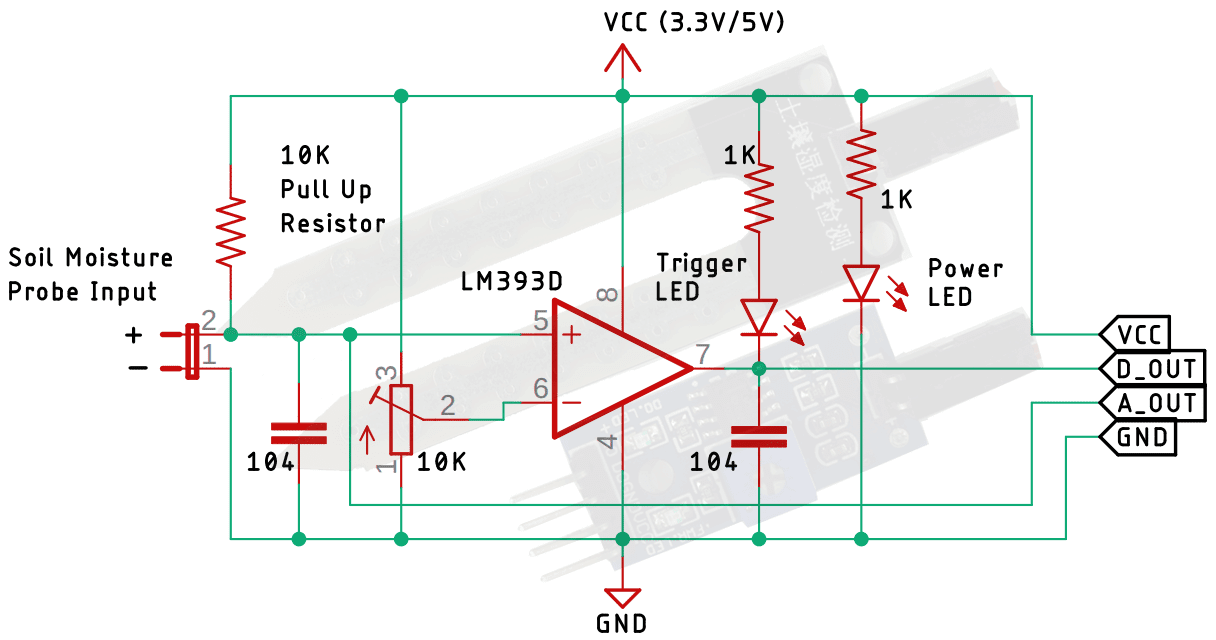
\includegraphics[width=1\textwidth]{images/image17.png}
    \caption{Soil Sensor Schematic}
    \label{fig:pic13}
\end{figure} 

\textbf{DC 3-6V Micro Submersible Water Pump} sucks water in from the side of the plastic casing and pushes it out the tubing port. The pump must be primed by keeping it inside water at all times.\\

\hspace{1cm}Specifications: 
\begin{itemize}[leftmargin=2cm]
    \item Operating Voltage: 3 to 6V
    \item Operating current: 130-200 mA
    \item Flow rate: 1,2-1,6L / min
\end{itemize}

\begin{figure}[ht]
    \centering
    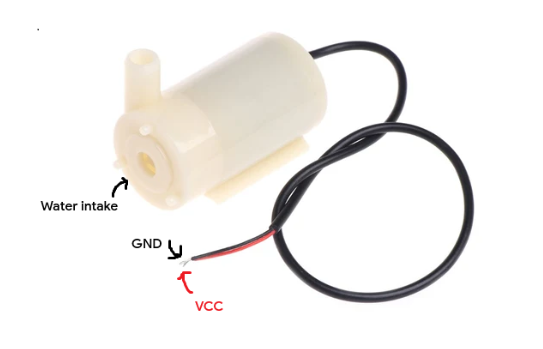
\includegraphics[width=0.7\textwidth]{images/image21.png}
    \caption{DC 3-6V Micro Submersible Water Pump}
    \label{fig:pic14}
\end{figure} 

\newpage

\begin{figure}[ht]
    \centering
    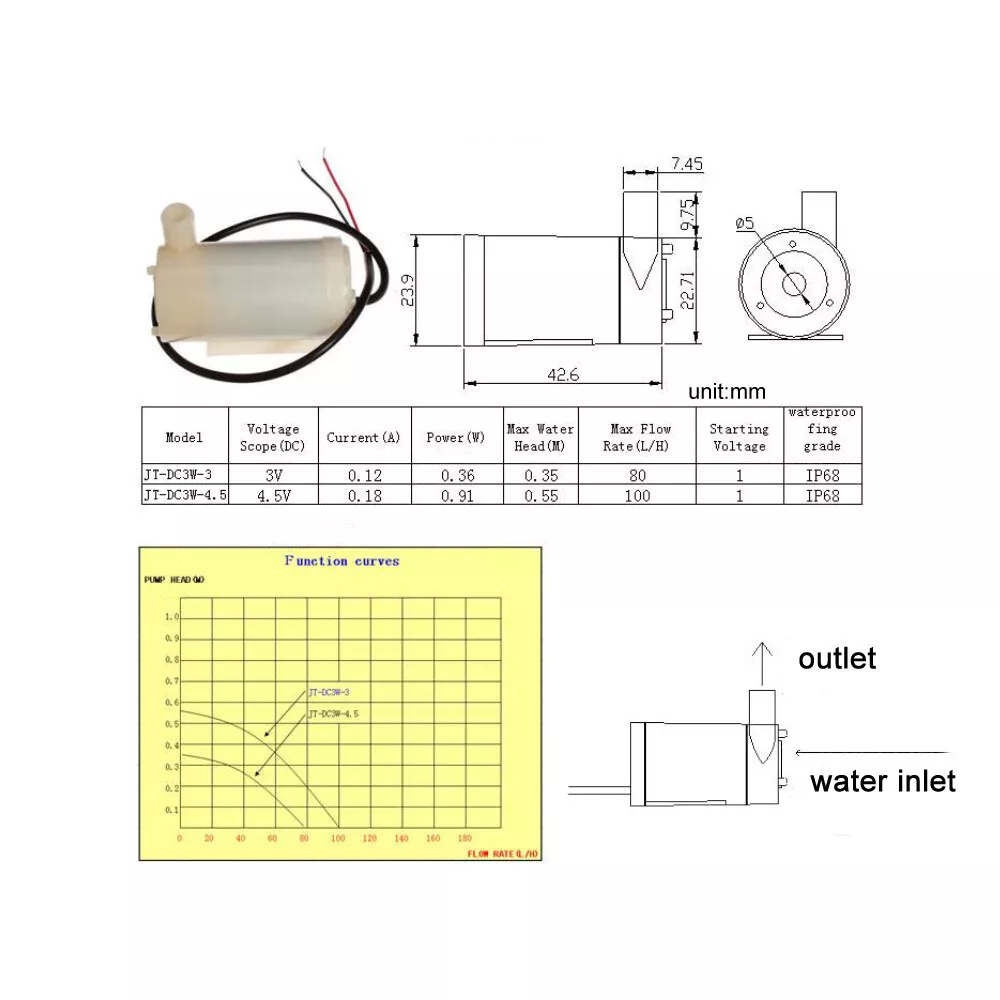
\includegraphics[width=1\textwidth]{images/image4.png}
    \label{fig:pic15}
\end{figure} 

\textbf{1 Channel 5V Relay Module} sucks water in from the side of the plastic casing and pushes it out the tubing port. The pump must be primed by keeping it inside water at all times.\\

\hspace{1cm}Specifications: 
\begin{itemize}[leftmargin=2cm]
    \item Operating Voltage: 5V
    \item Operating current: 15-20 mA
    \item Opto-Coupler isolation, for high voltage safety and prevent ground loop with microcontroller
\end{itemize}

\newpage

\begin{figure}[ht]
    \centering
    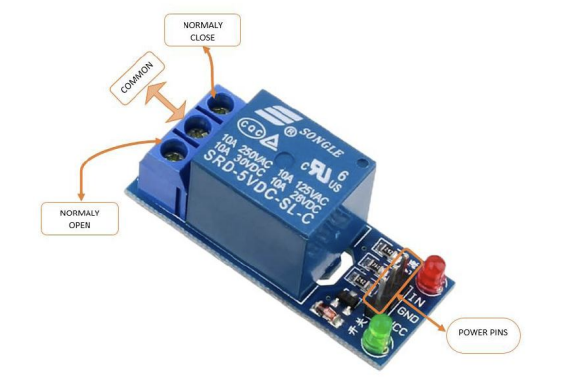
\includegraphics[width=0.85\textwidth]{images/image10.png}
    \caption{Relay Module Layout}
    \label{fig:pic16}
\end{figure} 

\begin{figure}[ht]
    \centering
    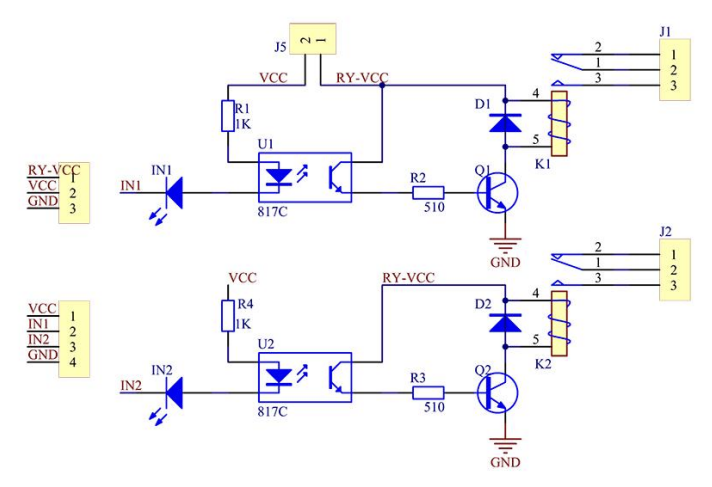
\includegraphics[width=0.8\textwidth]{images/image1.png}
    \caption{Relay Module Schematic}
    \label{fig:pic17}
\end{figure} 

\newpage

\textbf{5mm LED} is a small semiconductor device that emits light when an electric current passes through it. 

\hspace{1cm}Specifications: 
\begin{itemize}[leftmargin=2cm]
    \item Forward Voltage (VF): 1.8V to 2.4V
    \item Forward Current (IF): 30mA
\end{itemize}

\begin{figure}[ht]
    \centering
    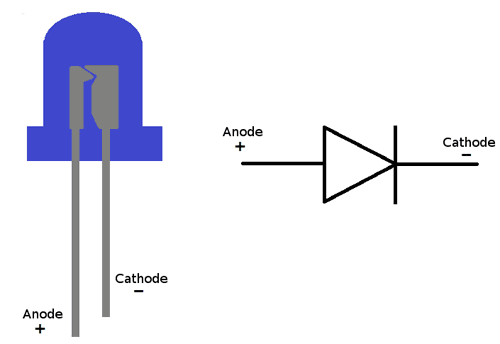
\includegraphics[width=0.9\textwidth]{images/image2.png}
    \caption{LED Pinout}
    \label{fig:pic18}
\end{figure} 

\newpage

\section{Programs, code}

\begin{figure}[ht]
    \centering
    
\includegraphics[width=0.9\textwidth]{images/image5.png}
    \label{fig:pic19}
\end{figure} 

Because the soil sensor is connected to GPIO21 and the 5V Relay to GPIO27 they are defined in 2 variables. Also the LEDs are connected to GPIO17 and GPIO4 so they are also taken and stored into 2 variables, one for each led.\\

\begin{figure}[ht]
    \centering
    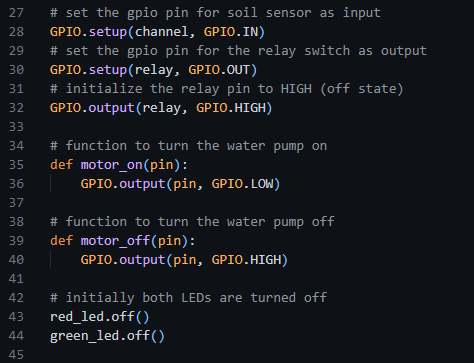
\includegraphics[width=0.9\textwidth]{images/image19.png}
    \label{fig:pic20}
\end{figure} 

\newpage

The GPIO for the soil sensor is set as input because information is taken from it and is used in the code. For 5v Relay the GPIO is set on output in order to send the signal from the code to it and then to the water pump
The initial value for 5V Relay is High meaning the off state for it (the relay is turned off). Both LEDs are initially turned off.\\

\begin{figure}[ht]
    \centering
    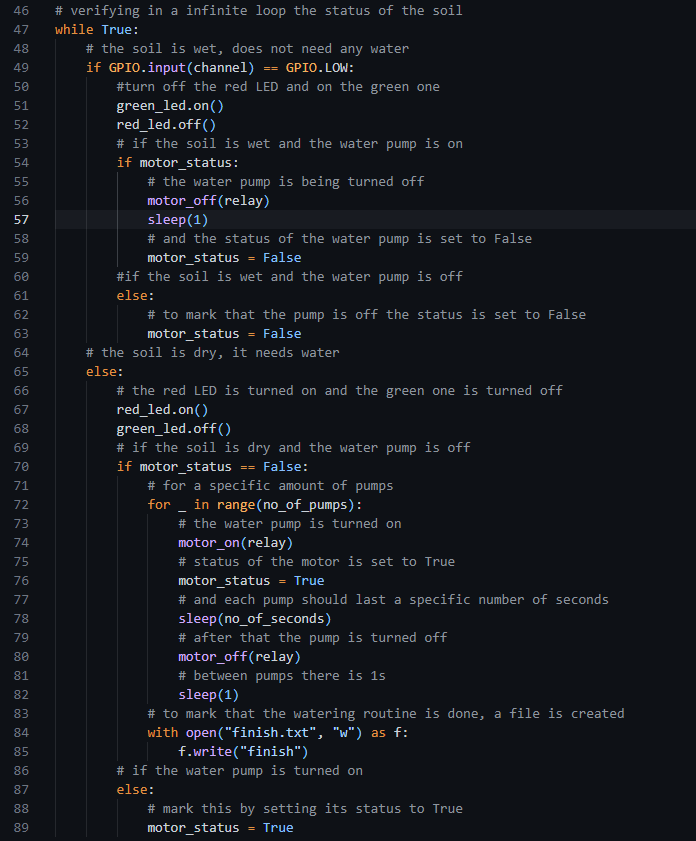
\includegraphics[width=0.9\textwidth]{images/image22.png}
    \label{fig:pic21}
\end{figure} 

In the above code, the soil sensor verifies constantly if the soil needs water and if it detects a low water level, the relay will be notified to turn on and after that the water pump, being connected to the 5v relay it will turn on and its status will be set to True. The Water pump will be on for a specific amount of pumps, each one a particular number of seconds depending on the user’s input. After that routine is finished the pump will be turned off and its status will be set to False because it is off.

\newpage


\nocite{*} % Include all entries from the .bib file


\bibliographystyle{plainnat} % Specify the bibliography style
\bibliography{references}


\end{document}